%%% template.tex
%%%
%%% This LaTeX source document can be used as the basis for your technical
%%% paper or abstract. Regardless of the length of your document, the commands
%%% are all the same.
%%% 
%%% The "\documentclass" command is the first command in your file. If you want to 
%%% prepare a version of your article with line numbers - a "review" version - 
%%% include the "review" parameter:
%%%    \documentclass[review]{acmsiggraph}
%%%

\documentclass{acmsiggraph}
\usepackage{subfigure}
\usepackage{algorithm}
\DeclareMathOperator*{\argmax}{argmax}
\DeclareMathOperator*{\argmin}{argmin}
%%% Title of your article or abstract.

\title{Coupled Joint Registration and Co-segmentation for Indoor Rigid Object Sets}
\author{Siyu Hu\thanks{e-mail:sy891228@mail.ustc.edu.cn}}
\pdfauthor{Siyu Hu}

%%% Used by the ``review'' variation; the online ID will be printed on 
%%% every page of the content.

\TOGonlineid{45678}

% User-generated keywords.

\keywords{Co-segmantion, Joint Registration}

% With the "\setcopyright" command the appropriate rights management text will be added
% to your document.

%\setcopyright{none}
%\setcopyright{acmcopyright}
%\setcopyright{acmlicensed}
\setcopyright{rightsretained}
%\setcopyright{usgov}
%\setcopyright{usgovmixed}
%\setcopyright{cagov}
%\setcopyright{cagovmixed}
%\setcopyright{rightsretained}

% The year of publication in the "\copyrightyear" command.

\copyrightyear{2016}

%%% Conference information, from the completed rights management form.
%%% The "\conferenceinfo" command has two parameters: 
%%%    - conference name
%%%    - conference date and location
%%% The "\isbn" field includes the year and month after the article ISBN.

\conferenceinfo{SIGGRAPH 2016 Posters}{July 24-28, 2016, Anaheim, CA} 
\isbn{978-1-4503-ABCD-E/16/07} 
\doi{http://doi.acm.org/10.1145/9999997.9999999}

\begin{document}

%%% This is the ``teaser'' command, which puts an figure, centered, below 
%%% the title and author information, and above the body of the content.

%\teaser{
%   \includegraphics[height=1.5in]{images/sampleteaser}
%   \caption{Spring Training 2009, Peoria, AZ.}
%}

\maketitle

\begin{abstract}

%In this sample paper, we describe the formatting requirements for
%content accepted to SIGGRAPH-sponsored events. The same format can be
%used for content ranging from a one- or two-page Poster or Talk abstract, to a
%full-length Technical Paper. 

%[New for 2016] Authors are now responsible for adding the appropriate rights management
%text to their final content, by adding information found on one's completed 
%rights management form to the source document.
%
%[New for 2016] Authors are now required to use ACM's current Computing Classification
%System for the inclusion of appropriate subject concepts.
%
%Please view the accompanying README file for a complete description of the formatting
%specifications.

\end{abstract}

%
% The code below should be generated by the tool at
% http://dl.acm.org/ccs.cfm
% Please copy and paste the code instead of the example below. 
%
\begin{CCSXML}
<ccs2012>
<concept>
<concept_id>10010147.10010371.10010382</concept_id>
<concept_desc>Computing methodologies~Image manipulation</concept_desc>
<concept_significance>500</concept_significance>
</concept>
<concept>
<concept_id>10010147.10010371.10010382.10010236</concept_id>
<concept_desc>Computing methodologies~Computational photography</concept_desc>
<concept_significance>300</concept_significance>
</concept>
</ccs2012>
\end{CCSXML}

\ccsdesc[500]{Computing methodologies~Image manipulation}
\ccsdesc[300]{Computing methodologies~Computational photography}

%
% End generated code
%

% The next three commands are required, and insert the user-generated keywords, 
% The CCS concepts list, and the rights management text.
% Please make sure there is a blank line between each of these three commands.

\keywordlist

\conceptlist

\printcopyright

\section{Introduction}
\label{sec:intro}
\mdf{In this paper, we present a new method to solve the object-level joint registration and co-segmentation problem. This problem originates from our attempt to build databases from scanned data.} \hsy{One reviewer said we should state this at the beginning of the introduction, he didn't understand our motivation until the late of introduction}
Many research projects and applications of indoor scenes require segmented, and even annotated 3D databases~\cite{SearchClassify,SceneFromExample,Fisher:2012:ESO:2366145.2366154,Chen:2014:ASM:2661229.2661239,Fisher:ActivityCentricSceneSynthesis}).
%
One way to build such a database is to interactively compose scenes using 3D object models, resulting in scenes with object segmentation and annotation naturally available, or to manually segment and annotate existing 3D scenes. 
%
This procedure can be tedious and time consuming, despite many efforts of improving the interaction experience~\cite{Merrell:2011:IFL:2010324.1964982, Xu:2013:SSC:2461912.2461968}.
%
Another way is to automatically generate scenes from 3D shape models according to images~\cite{Liu2015Model,Chen:2014:ASM:2661229.2661239}. 
%
In these methods, a retrieval procedure is usually needed and inevitably limit the result to a certain set of 3D models despite the actual 3D model in the input images.

Generating scene models directly from captured point clouds will significantly facilitate dataset construction and \mdf{increase} the dataset variety.
%
One of the major gaps between the required dataset and the available scene capturing frameworks~\cite{KinectFusion, dai2016bundlefusion} is the generic object-level segmentation. 
%
A generic object-level segmentation is not an equivalence of multi-label classification problem since it is not limited to a fixed number of objects in different scenes. 
%
Existing approaches for segmenting scanned 3D data require additional knowledge, such as the block-based stability~\cite{3DReasoningfromBlockstoStability}, or the motion consistency of rigid objects~\cite{Xu:2015:ACS:2816795.2818075}.  
%
%\cite{Xu:2015:ACS:2816795.2818075} proposes a practical and rather complete framework to close the gap between the required data set and available scene capturing method. 
%
%One of the observation in \cite{Xu:2015:ACS:2816795.2818075} is that the motion consistency of rigid object can serve as a strong evidence of general objectness.
While they employ a robot to do proactive push and use the movement tracking to verify and iteratively improve their object level segmentation result, \mdf{it remains significantly} challenging to recover the motion consistency in a \mdf{non-invasive} way.
\hsy{Without robot, our method is more tedious, since we need to schedule scanning every day.}


In this paper, we explore the motion consistency of rigid objects in a different aspect.
%
While the motion consistency of objects in indoor scenes is naturally revealed by human activities along the time, we hope to segment the objects in a scene from the scanned point clouds at different times. 
%
With respect to this idea, we are facing the choice of scanning schemes. 
%
One way is to record the change of the scene along with human activities.
Another option is to schedule a periodic sweep that only records the result of human activities but avoids the instants of human motion. 
%
The main challenge brought in by the second scheme is that we may not be able to solve the object correspondence by a local search due to the sparse sampling over time.
However, the very same challenge exists in the first scheme due to the occlusion caused by human bodies, not to mention other additional process (e.g. tracking with severe occlusions) needed for human bodies.
%
Therefore, we choose the second scheme.
\cxj{What is the advantage of the second scheme?} \hsy{Both schemes are difficult. We simply choose the less difficult one. The second scheme simply has less disadvantage.}
%
With the second scanning scheme, our original intention of building 3D scene datasets from canned data leads us to the problem of coupled joint registration and co-segmentation.


In this problem, registration and segmentation are entangled in each other. 
%
On one hand, the segmentation depends on the registration to connect the point clouds into series of rigid movement so that the object-level segmentation can be done based on the motion consistency. On the other hand, the registration depends on the segmentation to break the problem into a series of rigid joint registration instead of a joint registration with non-coherent point drift.
Non-coherent point drift means that a pair of points is close to each other in one point set, but their corresponding pair of points in another point set is far from each other. 
%
This happens when this pair of points actually belong to different objects.


We employ a group of Gaussian mixture models and each of these Gaussian mixture models represents a potential object. 
This model unentangle \cxj{Where do you find the word "unentangle"? did you create it?} \hsy{As verbs the difference between untangle and unentangle is that untangle is to remove tangles or knots while unentangle is to reverse the process of entanglement. Disentangle is to free something from entanglement.} the registration and segmentation in the way that the segmentation can be done by evaluate the probability of points belongs to the Gaussian mixture models and the registration can be done by evaluate rigid registration against each Gaussain mixture models.


In summary our work makes following contributions: 
\begin{enumerate}
	\item To the best of our knowledge, we first put forward the problem of joint registration and co-segmentation of point sets.
	
	\item We propose a generative model to simultaneously solve the joint registration and co-segmentation of point sets.
	
	\item We design a practical tool for efficient joint registration and co-segmentation based on the generative model. 
	
\end{enumerate}


\section{Related Work}
\label{sec:rw}
In this section we explain how our work is related to the previous work on point set processing and how we draw experiences from these methods. 

%\subsection{Point Set Registration with GMM Representation}
%\label{subsec:gmmreg}
\noindent{\textbf{Point Set Registration with GMM Representation.}}
There is a series of approaches that use Gaussian mixture model as \mdf{the} representation for point set registration problems \cxj{due to its general ability of representing point sets for both rigid and non-rigid registation}.
%
%
A \mdf{comprehensive} survey about approaches for point set registration using Gaussian mixture models can be found in \cite{GMM_PAMI}. 
They also present a unified framework for rigid and nonrigid registration problems. 
%
These methods select one of the point sets as the ``model'' and align other point sets with this \mdf{template}. \cxj{Is it better to use "template" than ``model''?} 
%
Myroeko and Song consider the registration of two point sets as a probability density estimation problem, and use Gaussian mixture model to represent the geometry and force the GMM centroids to move coherently as a group to preserve the topological structure of the point sets \cite{CPD}. This method is applicable to both rigid registration and non-rigid registration. \cxj{Does this method treat one point set as the template?}
%
As we highlighted in Sec.~\ref{sec:intro}, our problem is different from the non-rigid registration while the point drift is non-coherent in our \mdf{problem}.
%
Unlike these works, \cite{Evangelidis2014} treats all point sets equally.
They are all realizations of a Gaussian mixture model and the registration is cast into a clustering problem. 
A recent method pushes this idea to the application on a large scale dataset~\cite{GOGMA}. 
Comparing to these methods, our method can be seen as an extension of the formulation of \cite{Evangelidis2014} to simultaneously handle joint registration and co-segmentation. 
\cxj{It should not be a simple extension. You should highlight what is the most challeging part we solved compared with others. I would say: } \mdf{In comparison, we employ the same GMM representation of object models while we formulate the non-coherent point drift as .....  }

%\subsection{Image segmentation and co-segmentation}
%\label{subsec:coseg}
\noindent{\textbf{Image segmentation and co-segmentation}}
%
An influential work for interactive image segmentation is GrabCut~\cite{grabcut}. It uses two Gaussian mixture models, one for foreground and the other for background. 
To initialize these two Gaussian mixture models, a rectangle is manually placed to contain the foreground. 
Our design of interaction draws on the \mdf{experience} from \cite{grabcut}. 
%
The difference is that our interaction is designed for 3D space and can handle multi-object segmentation rather than foreground-background segmentation. 
%
\cite{Taniai_2016_CVPR} jointly recovers co-segmentation and dense per-pixel correspondences in two images. 
Its co-segmentation is limited to foreground-background segmentation. Our work solves a similar problem for multiple 3D point sets. 
\cxj{There are many image co-segmentation papers. If you want to discuss it, you should discuss more. }

\noindent{\textbf{Segmentation from Motion.}}
The idea that motion can be a strong hint for segmentation is used in many works.
\cite{Xu:2015:ACS:2816795.2818075} employs a robot to do proactive push and track the motion to learn object segmentation. 
\cite{unsupervisededge} exploits the motion in a video and uses the motion edges as the training data to learn an edge detector for image \cxj{use 'an image' or 'images'}. 
These methods lean on the motion that is continuous in time and can be tracked. Our method can handle motion that is not continuous in time.

\noindent{\textbf{3D Object Recognition based on Correspondence Grouping.}}
By allowing interactively input \mdf{the scene layout}, the joint registration and co-segmentation problem can be treated as a series of 3D object recognition problem in point sets. Our method should be classified as one of the correspondence grouping method. Comparing to previous methods \cxj{that uses ...}~\cite{hough,LOF}, our method simultaneously solve\mdf{s} the problem for multiple target models in multiple scenes.

\section{Method Overview}
\label{sec:method}
\subsection{Problem Statement}
Given series of point sets which record the same group of rigid indoor objects with different layout. We intend to samutaneously partition the point sets into objects and align the points of same object to recover layouts for corresponding object. Figure~\ref{fig:teaser} shows an example of input point clouds set.
\subsection{Basic Formulation}
To simutaneously model the joint registration and co-segmentation,  we come up with a generative model as follows:
\begin{equation}
\label{equ:model}
P(v_{mi})=\sum^{K_n}_{k=1}p_kN(v_{mi}|\phi_{mn}(x_k),\Sigma_k)
\end{equation}
which treat the i-th observed point $v_{mi}$ from the m-th point set as a sample point generated by one of $N$ object models.
We can define:\\
$$\Theta=\{\{p_k,x_k,\Sigma_k\}_{k=1}^{\sum{K_n}},\{\phi_{mn}\}_{m=1,n=1}^{MN}\}$$
as the parameter set of the generative model.\\
$p_k$ is the weight of the k-th Gaussian.\\
$x_k$ is the center of the k-th Gaussian.\\
$\Sigma_k$ is the standard deviation of the k-th Gaussian.\\
There are $K_{all}=\sum{K_n}$ Gaussian models in total and among them $K_n$ Gaussian models are treated as a group to represent n-th object.\\
$V$ is the set of M input point sets.\\
$v_{mi}$ is the i-th point of the m-th point cloud.\\
$\{\phi_{mn}\}$ are the functions of rigid transformation that transform the n-th group of gaussian centroids (representing the n-th object ) to the space of m-th input point sets.\\ 
Each object model is represented by a group of $K_n$ gaussian models.\\
Our goal of optimization is to maximize the probability of observed input sets sampled from the latent model.This problem can be solved in the framework of expectation-maximization. In particular, we bring in a latent parameter\\
$$Z=\{z_{mn}|m=1...M,n=1...N_m\}$$
such that $z_{mn}=k(k=1...\sum{K_n})$ assigns the observed point $v_{mi}$ to the k-th component of Gaussian mixture model. We aim to maximize the expected complete-data log-likelihood:
\begin{equation}
\label{equ:obj0}
f(\Theta|V,Z)=\mathbb{E}_Z[\ln P(V,Z;\Theta)|V]
\end{equation}
The object can be written as:
\begin{equation}
\label{equ:obj1}
\Theta=\arg\max{\sum_ZP(Z|V,\Theta)\ln{P(V,Z;\Theta)}}
\end{equation}
Such formulation can be seen as an adaption of joint registration formulation in \cite{Evangelidis2014}, upon which we seperate Gaussian models into groups to express multiple objects and the latent parameter  $Z$ that assign observed points to gaussian models can naturally indicate the object level segmentation.\\
By the asssumption of independent and identically distributed of input points, we can write the objective to:
\begin{equation}
\label{equ:obj2}
\Theta=\arg\max\sum_{mik}\alpha_{mik}(\ln p_k + \ln P(v_{mi}|z_{mi}=k;\Theta))
\end{equation}
where $\alpha_{mik} = P( z_{mi} = k | v_{mi} ; \Theta )$\\
By bringing in equation \ref{equ:model} and ingnoring constant terms, we can rewrite the objective as:
\begin{equation}
\label{equ:obj3}
\Theta=\arg\max\sum_{mik}\alpha_{mik}(||v_{mi}-\phi_{mn}(x_k)||_{\Sigma_k}^2 + \ln |\Sigma_k| - 2\ln p_k)
\end{equation}
where the $|\cdot|$ denotes the determinant and $||x||_A^2=x^TA^{-1}x$. It is predefined that $x_k$ is one of the gaussian centroid used to represent n-th object, which is why we apply transformation $\phi_{mn}$ on to the $x_k$. For the convenience of computation, we restrict the model to isotropic covariances, i.e.,$\Sigma_k=\sigma^2I$ and $I$ is the identity matrix.\\
Now, we can optimize this through iterating between estimating $\alpha_{mik}$ (Expectation-step) and maximizing $f(\Theta|V,Z)$ sequentially with respect to each parameters in $\Theta$ (Maximization-steps).
These steps are:\\
\textbf{E-step}:
this step estimates the posterior probability $\alpha_{mik}$ of $v_{mi}$ to be a point generated by the k-th Gaussian model.\\
\begin{equation}
\label{equ:estep}
\alpha_{mik}=\frac{p_k\sigma_k^{-3}exp(-\frac{1}{2\sigma_k^2}||v_{mi}-\phi_{mn}(x_k)||^2)}{\sum_s^{K_{all}}p_s\sigma_s^{-3}exp(-\frac{1}{2\sigma_s^2}||v_{mi}-\phi_{mn}(x_s)||^2)}
\end{equation}
\textbf{M-step-a}:this step update the transformations $\phi_{mn}$ that maximize $f(\Theta)$, given instant values for $\alpha_{mik}$, $x_k$, $\sigma_k$. We only consider rigid transformations, making  $\phi_{mn}(x)=R_{mn}x+t_{mn}$. The maximizer $R_{mn}^*,t_{mn}^*$  of $f(\Theta)$ is the same with the minimizers of the following constrained optimization problems:\\
\begin{equation}
\left\{
\begin{array}{rcl}
\min_{R_{mn},t_{mn}}&      &||(W_{mn}-R_{mn}X_n-t_{mn}\mathbf{e}^T)\Lambda_{mn}||_F^2\\
s.t.&      &R_{mn}^TR_{mn}=I, |R_{mn}|=1\\
\end{array} \right.
\end{equation}
where $\Lambda_{mn}$ is $K_n \times K_n$ diagonal matrix with elements $\lambda_{mnk}=\frac{1}{\sigma_k}\sqrt{\sum_i^{I_{m}}\alpha_{mik}}$,$I_m$ is the number of point for the m-th input point set, $X_n = [x_1,x_2,....,x_{K_n}]$ is the matrix stacked by the centroids of gaussian models that are predefined to represent the n-th object. $\mathbf{e}^T$ is a vector of ones, $||\cdot||_F$ denotes the Frobenius norm, and $W_{mn}=[w_{m1},w_{m2},...,w_{mk},...,w_{mK_n}]$, in which $w_{mk}$ is a weighted point as:\\
\begin{equation}
w_{mk}=\frac{\sum_{i=1}^{I_m}\alpha_{mik}v_{mi}}{\sum_{i=1}^{I_m}\alpha_{mik}}
\end{equation}
This problem have a similar solution of in \cite{Evangelidis2014}. The only difference is that we are estimating the transformation from latent models to the input point sets, since there are multiple group of $x_k$ corresponding to multiple objects in our latent model. The optimal can be given by:\\
\begin{equation}
R_{mn}^*=U_{mn}C_{mn}V_{mn}^T
\end{equation}
\begin{equation}
t_{mn}^*=\frac{1}{tr(\Lambda_{mn}^2)}(W_{mn}-R_{mn}X_n)\Lambda_{mn}^2\mathbf{e}
\end{equation}
where $[U_{mn},S,V_{mn}]=svd( W_{mn}\Lambda_{mn}P_{mn}\Lambda_{mn}X_{mn}^T )$ and $P_{mn}=I-\frac{\Lambda_{mn}\mathbf{e}(\Lambda_{mn}\mathbf{e})^T}{(\Lambda_{mn}\mathbf{e})^T\Lambda_{mn}\mathbf{e}}$,$I$ is identity matrix. $C_{mn}=diag(1,1,|U_{mn}||V_{mn}|)$.\\
\textbf{M-step-b}: this step we update the parameters related to the Gaussian mixture model. 
\begin{equation}
x_k^*=\frac{\sum_{m=1}^M\sum_{i=1}^{I_m}\alpha_{mik}(R_{mn}^{-1}v_{mi}-t_{mn})}{\sum_{m=1}^M\sum_{i=1}^{I_m}\alpha_{mik}}
\end{equation}
where $x_k$ is one of the Gaussian centroids that is predefined to represent n-th object. 
\begin{equation}
\sigma_k^{*2}=\frac{\sum_{m=1}^M\sum_{i=1}^{I_m}\alpha_{mik}||(v_{mi}-t_{mn}-R_{mn}^*x_k^*)||_2^2}{3\sum_{m=1}^M\sum_{i=1}^{I_m}\alpha_{mik}}
\end{equation}
\begin{equation}
p_k^*=\frac{\sum_{m,i}\alpha_{mik}}{M}
\end{equation}
\subsection{Bilateral Formulation}
When considering features, we can add bilateral terms into the generative model.
\begin{equation}
P(v_{mi},f_{mi})=\sum^{K_n}_{k=1}p_kN(v_{mi}|\phi_{mn}(xv_k),\sigma v_k)N(f_{mi}|xf_k,\sigma v_f)
\end{equation}
we measure the feature difference by a gaussian with diagnal $\Sigma$.
\subsection{Interaction Design}
Unfortunately, there are serveral parameters that can not be easily initialized in our formulation . In this subsection we first introduce our design of interaction, which is intuitive for users to input the semantic prior this way. We then explain how we can easily initlialize those parameters for our optimization based on the manual input.\\
As demonstrated in Figure~\ref{fig:interact}, we let user choose one of the point sets and placing and editing boxes in it to indicate the layout for this point set. From this, we can easily initialize the total number of objects $N$ and determine $\{K_n\}$ which is the numbers of Gaussian mixture models used to represent each object.
\begin{figure}[htb]
	\centering
	\includegraphics[width=.3\linewidth]{images/interact01.png}
	\includegraphics[width=.3\linewidth]{images/interact02.png}
	\includegraphics[width=.3\linewidth]{images/interact03.png}
	\includegraphics[width=.3\linewidth]{images/interact04.png}
	\includegraphics[width=.3\linewidth]{images/interact05.png}
	\includegraphics[width=.3\linewidth]{images/interact06.png}
	\caption{\label{fig:interact}
		From the first to the nineth, the nine images show the procedure of interaction:
		the user pick one point set and place boxes in it to indicate the layout for this point set. The box in white is the box currently under editing. The boxes in other colors are boxes placed to represent object layouts. One color represent one object. The interaction allows multiple boxes to represent same object.(e.g. the desk is represented by three boxes in same color)}
\end{figure}
These two paremeters are difficult to be initialized without semantic prior, but with the input of the users we can naturally initialize the $N$ as the number of different color label and the ${K_n}$ as 
\begin{equation}
K_n=\frac{V_n}{\sum V_n}K_{all}
\end{equation}
in which the $V_n$ represent the total volume of the boxes in the n-th color and the $K_{all}$ is initialized as $K_{all}=0.5*median(I_m)$ and $\{I_m\}$ are point numbers of $M$ input point set. This is an emperical choice borrowed from \cite{Evangelidis2014}.\\
The expectation maximizaton framework is easily converge to a local optimal. To cope with this problem we further use this interaction as a soft constraint to guide the optimization. Such constraint is done by simply altering the posterior probability $\alpha_{mik}$ as\\
\begin{equation}
\alpha_{mik}^*=\frac{\alpha_{mik}\beta_{mik}}{\sum_{i,k}\alpha_{mik}\beta_{mik}}
\end{equation}
where the $\beta_{mik}$ is the prior probability according to the boxes. It is defined as:\\
\begin{equation}
\beta_{mik}=\left\{
\begin{array}{rcl}
1&      & v_{mi} \in B_n\\
\exp(-\frac{\min_{v_{mj}}|| v_{mi} - v_{mj} ||_2^2  )}{C})&      &v_{mi} \notin B_n~and~v_{mj} \in B_n\\
\end{array} \right.
\end{equation}
where the $B_n$ is a point set that is enclosed by the boxes used to represent the layout of n-th object. The k-th Gaussian model is predefined to be one of the Gaussians used to represent n-th object. $\min_{v_{mj}}|| v_{mi} - v_{mj} ||_2^2$ is actually the squared euclidean distance from point $v_{mi}$ to the point set $B_n$, as we define the distance from a point to a point set as the minimum distance from the point to any point inside the point set. 



\section{Initialization and Optimization}
\label{sec:imp}
In this section, we summarize the entire framework for our algorithm and explain how do we intialize the parameters and guide the optimization with interaction.  
%
Based on our formulation in Sec.~\ref{sec:method}, our algorithm can be summarized as in Algorithm \ref{alg:jrcs}.
\begin{algorithm}[htb]
	\caption{Joint Registration and Co-segmentation (JRCS)}
	\label{alg:jrcs}
	\textbf{Input:}~~\\
	$\{\vb{V}_m\}$:$M$ 3D point sets\\
	$\Theta^0$:Initial parameters\\
	$\{\beta_{ik}\}_{m}$:layout based prior\\
	\textbf{Output:}~~\\
	$\Theta^q$:Final parameters~~
	\begin{enumerate}
		\item $q\leftarrow1$
		\item \textbf{repeat}
		\item E-step: Use $\Theta^{q-1}$ to estimate $\alpha_{mik}^q$ according to Eq.~(\ref{equ:estep}) (use Eq.~(\ref{equ:bestep}) for a bilateral formulation);
		\item Alter $\alpha_{mik}^q$ with $\{\beta_{ik}\}_{m}$ according to Eq.~(\ref{equ:alteralpha});
		\item M-step-a: use $\alpha^q_{mik}$, $\mathbf x^{q-1}_k$ to estimate $\{\mathbf{R}_{mn}^q\}$ and $\{\mathbf t_{mn}^q\}$ according to Eqs.~(\ref{equ:updateR})(\ref{equ:updatet});
		\item M-step-b: use $\alpha^q_{mik}$, $\{\mathbf{R}_{mn}^q\}$ and $\{\mathbf{t}_{mn}^q\}$ to update other parameters for Gaussian models according to Eqs.~ (\ref{equ:updatexk})(\ref{equ:updatesigma})(\ref{equ:updatepk})(\ref{equ:updatey})  (or use Eqs.~ (\ref{equ:updatefk})(\ref{equ:updatefsigma}) for a bilateral formulation);
		\item $q \leftarrow q+1$
		\item \textbf{until} Convergence \cxj{what is the convergence conditions?}
		\item \textbf{return} $\Theta^q$
	\end{enumerate}
\end{algorithm}

\subsection{Interaction}
\label{sec:imp:interact}
Unfortunately, there are a large number of parameters that can not be easily initialized in our formulation. 
%
In this subsection we first introduce our design of interaction, which is intuitive for users to input the semantic prior this way. We then explain how we can easily initialize those parameters for our optimization based on the manual input.


As demonstrated in Figure~\ref{fig:interact}, we let user choose one of the point sets and place boxes in it to indicate the layout for this point set. From this, we can easily initialize the total number of objects $N$ and determine $\{K_n\}$ which is the numbers of Gaussian mixture models used to represent each object.
\begin{figure}[htb]
	\centering
	\includegraphics[width=.3\linewidth]{images/interact01.png}
	\includegraphics[width=.3\linewidth]{images/interact02.png}
	\includegraphics[width=.3\linewidth]{images/interact03.png}
	\includegraphics[width=.3\linewidth]{images/interact04.png}
	\includegraphics[width=.3\linewidth]{images/interact05.png}
	\includegraphics[width=.3\linewidth]{images/interact06.png}
	\caption{\label{fig:interact}
		From the first to the sixth, the nine images show the procedure of interaction:
		the user pick one point set and place boxes in it to indicate the layout for this point set. The box in white is the box currently under editing. The boxes in other colors are boxes placed to represent object layouts. One color represents one object. The interaction allows multiple boxes to represents same object.(e.g. the desk is represented by three boxes in same color)}
\end{figure}
These two parameters are difficult to be initialized without semantic prior, but with the input of the users we can naturally initialize the $N$ as the number of different color label and the ${K_n}$ as 
\begin{equation}
\label{equ:K_n}
K_n=\frac{V_n}{\sum V_n}K_{all},
\end{equation}
in which the $V_n$ represent the total volume of the boxes in the $n^{th}$ color and the $K_{all}$ is initialized as $K_{all}=\frac{median(L_m)}{2}$ and $\{L_m\}$ are point numbers of $M$ input point sets. This is an empirical choice borrowed from \cite{Evangelidis2014}.\\
%
The expectation maximization framework is easily converged to a local optimal. To cope with this problem we further use this layout (boxes) from interaction as a soft constraint to guide the optimization and constrain the shape of generated object model. Such constraint is enforced by simply altering the posterior probability $\alpha_{mik}$ as
%
\begin{equation}
\label{equ:alteralpha}
\alpha_{mik}^*=\frac{\alpha_{mik}\beta_{mik}}{\sum_{i,k}\alpha_{mik}\beta_{mik}}
\end{equation}
where the $\beta_{mik}$ is the prior probability according to the boxes. It is defined as:
\begin{equation}
\beta_{mik}=\left\{
\begin{array}{rcl}
1& &\mathbf v_{mi} \in B_n\\
\exp(-\frac{\min_{\mathbf v_{mj}}|| \mathbf v_{mi} - \mathbf v_{mj} ||_2^2  )}{L})& &\mathbf v_{mi} \notin B_n~and~\mathbf v_{mj} \in B_n\\
\end{array} \right.
\end{equation}
where the $B_n$ is a point set that is enclosed by the boxes used to represent the layout of $n^{th}$ object. The $k^{th}$ Gaussian model is predefined to be one of the Gaussians used to represent $n^{th}$ object. $\min_{v_{mj}}|| v_{mi} - v_{mj} ||_2^2$ is actually the squared euclidean distance from point $v_{mi}$ to the point set $B_n$, as we define the distance from a point to a point set as the minimum distance from the point to any point inside the point set. $L$ here is a constant number with $L=2r^2$, and $r$ is the median of the radius of input point sets. The radius of a point set is half of length of diagonal line of its axis-aligned bounding box.   
\begin{figure}[htb]
	\centering
	\includegraphics[width=\linewidth]{images/localoptimal/localoptimal}
	\caption{\label{fig:localoptimal}This figure shows an example result when converges to a local optimal. (a) is the result of segmentation of this local optimal. (b) is the final centroids of latent model. It shows that from top to down the 2nd and 3rd object model both include part of the table and part of the chair.}
\end{figure}
This alteration on posterior probability is only done with the probability related to the $m^{th}$ point set that have the mannual input layout (the boxes) in it. This alteration can help prevent the optimization from converging to a local optimal as in Figure~\ref{fig:localoptimal}. The result from the Figure~\ref{fig:localoptimal} has the same input and initialization with the result from Figure~\ref{fig:teaser}, but it does not use the posterior alteration as a soft constraint.

\subsection{Initialization}
%
\textbf{Initialization of $\Theta$}: We start with determining the total number of Gaussian model $K_{all}$ as we explained in Sec.~\ref{sec:imp:interact}.
We set $p_k=\frac{1}{\sum K_n}$, which means each Gaussian has the same weight at the beginning. 
%
We separate the total $K_{all}$ Gaussian models into $N$ groups to represent $N$ objects. 
%
Each group has $K_n$ Gaussian models based on Eq.~(\ref{equ:K_n}). 
We implement this by recording the start and end indices of the $N$ objects. In other words, we record
$\{0,K_1,K_1+1,K_1+K_2,...,\sum^{N-1}K_n+1,\sum^N K_n\}$. $\{\vb{x}_k\}_n$ are Gaussian centroids of $n^{th}$ group and they are initialized as a random positions uniformly distributed on the surface of a sphere, whose radius $r$ is chosen as the median of the radius of the input point sets. 
%
The center of the $n^{th}$ sphere is $\vb{c}_n=(0,0,z_n)$, where $z_n\in \{-(N-1)r,-(N-3)r,...,(N-1)r\}$.\cxj{What is N? In total, there would be $2N-1$ centers?} \hsy{No, The common difference is $2r$ here. it is $\{-2r,0,2r\}$ when $N=3$ and $\{-3r,-r,r,3r\}$ when $N=4$}
%
This means that the object models are vertically arranged in latent space as shown in Figure~\ref{fig:teaser}(c) and in Figure~\ref{fig:localoptimal}(b). 
We choose vertical arrangement for groups of object merely for the convenience of visualization. \cxj{So you can also set the spheres horizontally or slantly or arbitrarily for registration only?}
%
We choose spheres as the initial shape so that we can initialize all the $\mathbf{R}_{mn}$ to identity matrix. 
%
For the $\vb{t}_{mn}$ we initialize them as $\mathbf{t}_{mn}=- \mathbf{c}_n$ so that all the object model starting with position at origin point when they are transformed to the space of each input set. 
%
However, if the $m^{th}$ input point set has the manually placed layout, we treat the associated $\mathbf{t}_{mn}$ differently. For this case we have:
\begin{equation}
	\label{equ:initt}
	\vb{t}_{mn}=\frac{\sum_{\vb{v}_{mi} \in B_n}\vb{v}_{mi}}{N(B_n)}-\vb{c}_n
\end{equation}
where $N(B_n)$ here is the number of element in $B_n$ and $B_n$ is the point set that is enclosed by the manually input layout (box) \mdf{indicating arrangement of the $n^{th}$ object}. 
\cxj{You have many boxes, $B_n$ is which one?. The number $n$ is also confusing while you use $n$ for sphere center index.} \hsy{ $n$ is always indices for object and $B_n$ is the box for $n^{th}$ object }
\subsection{Hot Intervention Mechanism}
\cxj{I am curious where do you get this word? Any reference?}
%
Our current implementation of optimization is quite slow (fails to converge in an interactive-rate time) especially when the numbers of points inside the input point sets are large and it is possible for our optimization to stuck in a local optimal, requiring the guide from the manual input. 
%
As a compensation for these drawbacks, we implement a hot intervention mechanism, allowing the manual input to take effect during the optimization process. 
Theoretically, this is possible due to the i.i.d assumption, under which the calculation of posterior probability is independent for each input point set. 
%
Even after the optimization is started, we can still allow the user to add more layouts \cxj{what do you mean by 'add layouts'?} for other point sets and the program can do the same alteration as (\ref{equ:alteralpha}) in the next iteration. 
%
Figure~\ref{fig:hi} shows how the users can use the hot intervention mechanism within our tool.
%
\begin{figure}[htb]
	\centering
	\includegraphics[width=\linewidth]{images/hotintervention/hi}
	\caption{\label{fig:hi} This figure shows the hot intervention mechanism. (a) The input point sets with manually placed layout in the $2^{nd}$ point set. (b) For each iteration, the instant segmentation results for all point sets are shown in the blue region while the object models (the shape of the centroids of the Gaussian models) are shown in the red region. (c) The user picks another input point set and adds more boxes targeting the incorrect segmentation to further guide the optimization when the optimization is running. \cxj{highlight the newly added box. Do not show the entire interface.. just show the data. }}
\end{figure}
\section{Experiments and Discussion}
\label{sec:exp}
\subsection{Debugging The Smooth Step}
%\textbf{Bug Description:}\\
%When the smooth step is added, the mixture of gaussian model won't expand to fit the input observations.\\
%\textbf{Test Case Generation:}\\
%In order to debug the problem, I generated a set of six synthetic point clouds. For the purpose of debugging, I deliberately made sure that the first 2657 points belonging to table, the following 2028 points belonging to chair, the last 3286 points belonging to teddy. The Test Cases are shown in Figure \ref{fig:syn-data}.
%\begin{figure}[ht]
%  \centering
%  \includegraphics[width=3.0in]{images/synthetic_data}
%  \caption{The Synthetic Data for Test:they are composed of three objects (teddy table and chair) with different rigid motion}
%  \label{fig:syn-data}
%\end{figure}\\
%\textbf{The Example of $\alpha$:}\\
%The $\alpha$ are caculated as
%$$\alpha_{ijk}=p_np_kN(\phi_n(v_{ij})|x_k,\Sigma_k)$$
%The example $\alpha$ with no smooth:\\
%\begin{figure*}
%\centering
%	\subfigure[
%	$\alpha_0$,iteration 0
%	]{\label{fig:a0_0}
%		
\includegraphics[width=0.3\textwidth]{images/alpha_0_iter_0.png}}
%	\subfigure[
%	$\alpha_0$,iteration 9
%	]{\label{fig:a0_9}
%		
\includegraphics[width=0.3\textwidth]{images/alpha_0_iter_9.png}}
%	\subfigure[
%	$\alpha_0$,iteration 19
%		]{\label{fig:a0_19}
%		
\includegraphics[width=0.3\textwidth]{images/alpha_0_iter_19.png}}
%	\subfigure[
%		$\alpha_1$,iteration 19
%		]{\label{fig:a1_19}
%		
\includegraphics[width=0.18\textwidth]{images/alpha_1_iter_19.png}}
%	\subfigure[
%		$\alpha_2$,iteration 19
%		]{\label{fig:a2_19}
%		
\includegraphics[width=0.18\textwidth]{images/alpha_2_iter_19.png}}
%	\subfigure[
%		$\alpha_3$,iteration 19
%		]{\label{fig:a3_19}
%		
\includegraphics[width=0.18\textwidth]{images/alpha_3_iter_19.png}}
%	\subfigure[
%		$\alpha_4$,iteration 19
%		]{\label{fig:a4_19}
%		
\includegraphics[width=0.18\textwidth]{images/alpha_4_iter_19.png}}
%	\subfigure[
%		$\alpha_5$,iteration 19
%		]{\label{fig:a5_19}
%		
\includegraphics[width=0.18\textwidth]{images/alpha_5_iter_19.png}}
%	\caption{$\alpha$ with no smooth}
%	\label{fig:a_no_smooth}
%\end{figure*}
%as shown in Figure~\ref{fig:a_no_smooth}\\
%\textbf{The Problematic $\alpha$}
%\begin{figure*}
%	\centering
%	\subfigure[
%	$\alpha_0$,iteration 0
%	]{\label{fig:a0_0_smooth}
%		\includegraphics[width=0.3\textwidth]{images/alpha_0_iter_0_smooth.png}}
%	\subfigure[
%	$\alpha_1$,iteration 0
%	]{\label{fig:a1_0_smooth}
%		\includegraphics[width=0.3\textwidth]{images/alpha_1_iter_0_smooth.png}}
%	\caption{$\alpha$ after smooth}
%	\label{fig:a_smooth}
%\end{figure*}
\subsection{Current Result}
%As shown in Figure~\ref{fig:current_result}
%\begin{figure*}
%	\centering
%	\includegraphics[width=\textwidth]{images/result_iter_18.png}
%	\caption{Current Result}
%	\label{fig:current_result}
%\end{figure*}\\
%\textbf{Current Alpha}\\
%\begin{figure*}
%	\centering
%	\subfigure[
%	$\alpha_0$,iteration 0
%	]{\label{fig:a0_0_0427}
%		\includegraphics[width=0.3\textwidth]{images/alpha_0_iter_0_0427.png}}
%	\subfigure[
%	$\alpha_0$,iteration 9
%	]{\label{fig:a0_9_0427}
%		\includegraphics[width=0.3\textwidth]{images/alpha_0_iter_9_0427.png}}
%	\subfigure[
%	$\alpha_0$,iteration 19
%	]{\label{fig:a0_19_0427}
%		\includegraphics[width=0.3\textwidth]{images/alpha_0_iter_19_0427.png}}
%	\subfigure[
%	$\alpha_0$,iteration 0 smooth
%	]{\label{fig:a0_0_0427_smooth}
%		\includegraphics[width=0.3\textwidth]{images/alpha_0_iter_smooth_0_0427.png}}
%	\subfigure[
%	$\alpha_0$,iteration 9 smooth
%	]{\label{fig:a0_9_0427_smooth}
%		\includegraphics[width=0.3\textwidth]{images/alpha_0_iter_smooth_9_0427.png}}
%	\subfigure[
%	$\alpha_0$,iteration 19 smooth
%	]{\label{fig:a0_19_0427_smooth}
%		\includegraphics[width=0.3\textwidth]{images/alpha_0_iter_smooth_19_0427.png}}
%	\caption{$\alpha$ after smooth}
%	\label{fig:current_alpha}
%\end{figure*}
\subsection{Initialization Experiments}
%\begin{figure*}
%	\centering
%	\includegraphics[width=\textwidth]{images/init_input.png}
%	\caption{Input for Initialization Experiments}
%	\label{fig:input_for_init}
%\end{figure*}
%\begin{figure*}
%	\centering
%	\includegraphics[width=\textwidth]{images/init_seg.png}
%	\caption{Segmentation for Initialization Experiments}
%	\label{fig:seg_for_init}
%\end{figure*}
%\begin{figure*}
%	\centering
%	\includegraphics[width=\textwidth]{images/init_cluster.png}
%	\caption{Clustering for Initialization Experiments}
%	\label{fig:cluster_for_init}
%\end{figure*}


%Ut sagittis arcu ut turpis sodales, nec venenatis magna efficitur. Fusce non rhoncus risus, ac tincidunt arcu. Nulla lacus odio, accumsan tempor dolor sit amet, tincidunt porttitor justo. Quisque vulputate ex ac purus ultrices tristique. Pellentesque habitant morbi tristique senectus et netus et malesuada fames ac turpis egestas. Curabitur sed ullamcorper metus. Phasellus eu purus eget leo vulputate auctor vel scelerisque velit.

%\begin{table}[ht]
%  \centering
%  \caption{A simple table.}
%  \begin{tabular}{|r|l|}
%    \hline
%    7C0 & hexadecimal \\
%    3700 & octal \\ \cline{2-2}
%    11111000000 & binary \\
%    \hline \hline
%    1984 & decimal \\
%    \hline
%  \end{tabular}
%\end{table}
  
%Etiam sed mattis justo. Mauris lorem sapien, pellentesque vel viverra varius, porta ut nisi. Cras vel interdum dui, vitae fermentum elit. Nulla eu libero finibus, bibendum elit nec, ullamcorper velit. Donec ultrices, purus id ullamcorper euismod, ipsum erat sodales augue, ut sagittis sapien magna nec ex. Nulla massa arcu, suscipit non molestie ut, tristique id tellus. Maecenas nec malesuada mauris, vitae mattis sem. Quisque at risus quis arcu eleifend lacinia non sed neque.

%\section{Second Section Heading}

%Ut sagittis arcu ut turpis sodales, nec venenatis magna efficitur. Fusce non rhoncus risus, ac tincidunt arcu. Nulla lacus odio, accumsan tempor dolor sit amet, tincidunt porttitor justo. Quisque vulputate ex ac purus ultrices tristique. Pellentesque habitant morbi tristique senectus et netus et malesuada fames ac turpis egestas. Curabitur sed ullamcorper metus. Phasellus eu purus eget leo vulputate auctor vel scelerisque velit.

%\subsection{This is a subsection}

%Nunc vitae lorem nec diam ultrices fringilla. Aliquam volutpat metus ut magna bibendum, sed ultricies nunc placerat. Nulla volutpat rutrum vehicula. Cum sociis natoque penatibus et magnis dis parturient montes, nascetur ridiculus mus. Aliquam vel ligula elit. Nulla fermentum purus eu venenatis mollis. Nulla placerat dui accumsan urna pharetra maximus. Sed nec orci arcu. Suspendisse faucibus blandit libero ut feugiat. Nulla vitae imperdiet nulla. Cum sociis natoque penatibus et magnis dis parturient montes, nascetur ridiculus mus.

%Etiam sed mattis justo. Mauris lorem sapien, pellentesque vel viverra varius, porta ut nisi. Cras vel interdum dui, vitae fermentum elit. Nulla eu libero finibus, bibendum elit nec, ullamcorper velit. Donec ultrices, purus id ullamcorper euismod, ipsum erat sodales augue, ut sagittis sapien magna nec ex. Nulla massa arcu, suscipit non molestie ut, tristique id tellus. Maecenas nec malesuada mauris, vitae mattis sem. Quisque at risus quis arcu eleifend lacinia non sed neque.

%\subsection{This is another subsection}

%Praesent lacinia, risus eget lacinia elementum, lorem elit ullamcorper arcu, quis condimentum ipsum dui at felis. Mauris maximus at lectus condimentum efficitur. Maecenas luctus, magna nec porttitor semper, justo libero semper nisi, nec commodo nunc turpis a velit. Morbi ac elementum urna, in elementum massa. Mauris ipsum turpis, fringilla in pellentesque a, mattis non erat. Cras vitae sodales lacus. Mauris sit amet laoreet ipsum. Maecenas quis consectetur dui. Nunc vulputate, dui eu blandit volutpat, augue dui molestie risus, et viverra lorem ligula quis eros.

%\begin{figure}[ht]
%  \centering
%  \includegraphics[width=3.0in]{images/ferrari_laferrari}
%  \caption{Ferrari LaFerrari. Image courtesy Flickr user ``gfreeman23.''}
%  \label{fig:ferrari}
%\end{figure}
%
%\section{Third Section Heading}

%Ut sagittis arcu ut turpis sodales, nec venenatis magna efficitur. Fusce non rhoncus risus, ac tincidunt arcu. Nulla lacus odio, accumsan tempor dolor sit amet, tincidunt porttitor justo. Quisque vulputate ex ac purus ultrices tristique. Pellentesque habitant morbi tristique senectus et netus et malesuada fames ac turpis egestas. Curabitur sed ullamcorper metus. Phasellus eu purus eget leo vulputate auctor vel scelerisque velit.

%Nunc vitae lorem nec diam ultrices fringilla. Aliquam volutpat metus ut magna bibendum, sed ultricies nunc placerat. Nulla volutpat rutrum vehicula. Cum sociis natoque penatibus et magnis dis parturient montes, nascetur ridiculus mus. Aliquam vel ligula elit. Nulla fermentum purus eu venenatis mollis. Nulla placerat dui accumsan urna pharetra maximus. Sed nec orci arcu. Suspendisse faucibus blandit libero ut feugiat. Nulla vitae imperdiet nulla. Cum sociis natoque penatibus et magnis dis parturient montes, nascetur ridiculus mus.

%Etiam sed mattis justo. Mauris lorem sapien, pellentesque vel viverra varius, porta ut nisi. Cras vel interdum dui, vitae fermentum elit. Nulla eu libero finibus, bibendum elit nec, ullamcorper velit. Donec ultrices, purus id ullamcorper euismod, ipsum erat sodales augue, ut sagittis sapien magna nec ex. Nulla massa arcu, suscipit non molestie ut, tristique id tellus. Maecenas nec malesuada mauris, vitae mattis sem. Quisque at risus quis arcu eleifend lacinia non sed neque.

\section*{Acknowledgements}

To Robert, for all the bagels.

\bibliographystyle{acmsiggraph}
\nocite{*}
\bibliography{JRCS}
\end{document}
